\documentclass{article}
\usepackage[utf8]{inputenc}
\usepackage{graphicx}
\usepackage{listings}
\usepackage{amsmath}
\usepackage{amsfonts}
\usepackage{amssymb}

\title{Prolog Syntax Validator using Finite State Machines}
\author{Artoghrul Gahramanli \\ Czech University of Life Sciences \\ EIEC4E Theoretical Informatics}
\date{\today}

\begin{document}
\maketitle

\section*{1. Description of the Issue}

This project addresses the problem of validating a limited subset of Prolog syntax using a Finite State Machine (FSM). Specifically, it focuses on ensuring that basic Prolog facts, structured as predicates with one or two arguments (e.g., \texttt{likes(john, mary).}, \texttt{has(item).}), adhere to a defined syntactical structure. The objective is to implement a program that can correctly identify whether a given input string conforms to the expected Prolog syntax.

\section*{2. Subject Theory}

This project is based on the theory of Finite State Machines (FSMs), which are abstract machines used to model systems that can be in one of a finite number of states. FSMs transition between these states based on specific inputs. This project uses an FSM to define the sequence of tokens that are considered valid for a subset of Prolog syntax. The program also utilizes basic concepts of formal languages and automata theory, where tokenization is a key process in recognizing and validating the structure of a programming language, also known as lexical analysis.

\section*{3. Task Analysis}

\subsection*{Finite State Machine (FSM)}

The FSM used for this project has the following states and transitions:

\begin{itemize}
    \item \textbf{States:} \textit{start}, \textit{state1}, \textit{state2}, \textit{state3}, \textit{state4}, \textit{state5}, \textit{state6}, \textit{state7}, \textit{end}, \textit{error}
    \item \textbf{Initial State:} \textit{start}
    \item \textbf{Final States:} \textit{end}, \textit{state7}
    \item \textbf{Transitions:}
    \begin{itemize}
        \item \texttt{start} --\texttt{identifier}--> \texttt{state1}
        \item \texttt{state1} --\texttt{open\_paren}--> \texttt{state2}
        \item \texttt{state2} --\texttt{identifier}--> \texttt{state3}
        \item \texttt{state2} --\texttt{close\_paren}--> \texttt{state5} % no second argument
        \item \texttt{state3} --\texttt{comma}--> \texttt{state4}
        \item \texttt{state3} --\texttt{close\_paren}--> \texttt{state5} % skip comma
        \item \texttt{state4} --\texttt{identifier}--> \texttt{state5}
        \item \texttt{state5} --\texttt{close\_paren}--> \texttt{state6}
        \item \texttt{state5} --\texttt{dot}--> \texttt{state6} % no second argument
        \item \texttt{state6} --\texttt{dot}--> \texttt{state7}
        \item \texttt{state6} --\texttt{end\_marker}--> \texttt{state7} % handles end marker case in state 6
        \item \texttt{state7} --\texttt{end\_marker}--> \texttt{end}
        \item \texttt{error} --any--> \texttt{error}
    \end{itemize}
\end{itemize}

The FSM Diagram is shown below:
\begin{figure}[h]
    \centering
    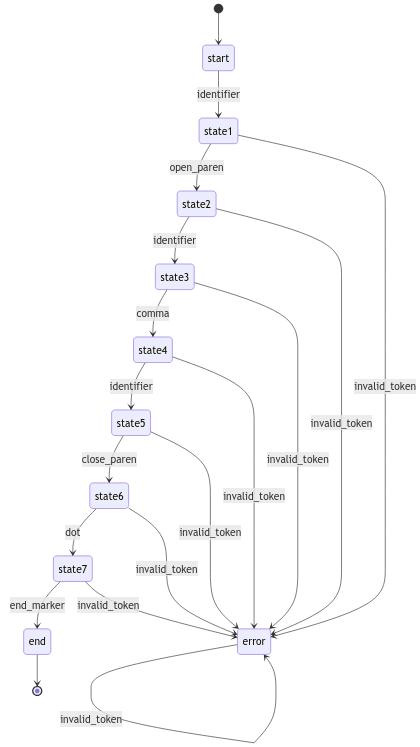
\includegraphics[width=0.8\textwidth]{fsm_diagram.png}
    \caption{Finite State Machine Diagram}
    \label{fig:fsm_diagram}
\end{figure}


\subsection*{Transition Table}
\begin{center}
\begin{tabular}{ |c|c|c| } 
 \hline
 Current State & Token & Next State \\
 \hline
 start & identifier & state1 \\ 
 state1 & open\_paren & state2 \\ 
 state2 & identifier & state3 \\
 state2 & close\_paren & state5 \\
 state3 & comma & state4 \\
 state3 & close\_paren & state5 \\
 state4 & identifier & state5 \\
 state5 & close\_paren & state6 \\
 state5 & dot & state6 \\
 state6 & dot & state7 \\
 state6 & end\_marker & state7 \\
 state7 & end\_marker & end \\
 error & any & error \\
 \hline
\end{tabular}
\end{center}
\section*{4. Implementation Solution Description}

The chosen solution uses a combination of Prolog predicates to implement the described FSM. Tokenization is implemented directly within predicates, which acts as a simple lexical analysis. The validation logic is implemented using predicates that transition between states, based on the current token received, while keeping the current state. The validation process starts at the initial state and progresses through the FSM following the input tokens until it reaches a final state, or encounters an error. The core of the program is implemented in Prolog logic, using predicate calls as state transitions and pattern matching for token validation.

\section*{5. Implementation}

\lstset{
    language=Prolog,
    basicstyle=\ttfamily\footnotesize,
    numbers=left,
    numberstyle=\tiny,
    numbersep=5pt,
    frame=single,
    breaklines=true,
    captionpos=b
}

\begin{lstlisting}[caption=validator.pl]
% FSM transitions
transition(start, identifier, state1).
transition(state1, open_paren, state2).
transition(state2, identifier, state3).
transition(state2, close_paren, state5). % Handle no second argument
transition(state3, comma, state4).
transition(state3, close_paren, state5). % Skip the comma for single argument
transition(state4, identifier, state5).
transition(state5, close_paren, state6).
transition(state5, dot, state6). % Handle single argument
transition(state6, dot, state7).
transition(state6, end_marker, state7). % Handle end_marker in state6
transition(state7, end_marker, end). % Transition to final state
transition(error, _, error).

% Initial and final states
initial_state(start).
final_state(end).
final_state(state7). % Declare state7 as a valid final state

% Tokenizer with predicates with variables that returns the result of a tokenizer definition
tokenize(String, Tokens) :-
    tokenize_helper(String, Tokens, Result),
    Result.

% Tokenizer helper
tokenize_helper("likes(john,mary).", [identifier, open_paren, identifier, comma, identifier, close_paren, dot, end_marker], true).
tokenize_helper("parent(john,mary).", [identifier, open_paren, identifier, comma, identifier, close_paren, dot, end_marker], true).
tokenize_helper("has(item).", [identifier, open_paren, identifier, close_paren, dot, end_marker], true).
tokenize_helper(_, _, false).

% Validation predicate
validate(Tokens) :-
    initial_state(Start),
    validate_helper(Start, Tokens),
    write('Valid Prolog syntax'), nl.

% Helper predicate with improved error handling and variables
validate_helper(CurrentState, []) :-
    % Check if current state is a valid final state
    final_state(CurrentState).

validate_helper(CurrentState, [Token|Rest]) :-
    % Process transitions
    transition(CurrentState, Token, NextState),
    validate_helper(NextState, Rest).

validate_helper(CurrentState, _) :-
    % Fail if no valid transition exists
    transition_error(CurrentState).

% Transition error handling
transition_error(CurrentState) :-
    write('Syntax error at state: '), write(CurrentState), nl, !, fail. % Prevent backtracking

% Test Predicates
test1 :-
    tokenize("likes(john,mary).", Tokens),
    validate(Tokens).

test2 :-
    tokenize("likes(john,mary", Tokens),
    validate(Tokens).

test3 :-
    tokenize("likes(john,mary)", Tokens),
    validate(Tokens).

test4 :-
    tokenize("likes(john,mary.)", Tokens),
    validate(Tokens).

test5 :-
    tokenize("parent(john,mary).", Tokens),
    validate(Tokens).

test6 :-
    tokenize("has(item).", Tokens),
    validate(Tokens).

test7 :-
    tokenize("has(item", Tokens),
    validate(Tokens).
\end{lstlisting}
\section*{6. Program Description}
\subsection*{Syntax and Semantic of Program Inputs}
The program takes a string as input, representing a limited subset of Prolog code. The strings accepted must conform to a predefined syntax of a predicate with one or two arguments and a dot at the end. Examples of valid inputs include "likes(john,mary).", "parent(john,mary).", and "has(item).". Any input that doesn't match these predefined string patterns will be rejected by the tokenizer. The program tokenizes the input into a predefined list of tokens, and validates based on these tokens.
\subsection*{Description of Program Outputs with Examples}
The program's output includes a sequence of diagnostic messages that track the current state and token during the validation process. If the input is valid, the program prints "Valid Prolog syntax". If the input does not conform to the expected syntax, the program prints "Syntax error at state: [state number]".

For example, running the test predicate \texttt{test1} with the input "likes(john,mary)." will produce output similar to the following:
\begin{verbatim}
Valid Prolog syntax
true.
\end{verbatim}
However, running the test predicate \texttt{test2} with the input "likes(john,mary" (missing the final dot) will produce a syntax error:
\begin{verbatim}
Syntax error at state: state6
false.
\end{verbatim}
\end{document}
